\documentclass[../proyecto.tex]{memoir}

\begin{document}

\chapter{Metodología}
\section{Representación del juego de vida de Conway}

Fijada una configuración inicial $z$, enteremos por ejecución o simulación del juego de vida de Conway de duración $n \in \mathds{N} \cup \{ \infty\}$ al resultado de aplicar $n$ veces la función de transición global del juego de vida de Conway a la configuración inicial y lo notaremos $C_{n}(z)$. Sea $t$ tal que $1 \leq t \leq n$, diremos que es el instante $t$ de la ejecución/simulación/experimento del juego de vida de Conway de duración $t$, el resultado de aplicar $t$ veces la función de transición global a una configuración inicial $z$ y lo notaremos $C^t_n(z)$. Por último, los conjuntos de puntos $C^{t'}_{n'}(z')$, $C^{t}_{n}(z)$ si los conjuntos de células de cada simulación son idénticos. De la misma manera, entederemos por ejecución o simulación del juego de vida de Conway $\alpha$-asíncrono de duración $n$ al resultado de aplicar $n$ veces la función de transición global a la configuración inicial $z$ y lo notaremos $C_{n}(z)(\alpha)$ donde $\alpha$ es un número real en el intervalo $(0,1)$.

Como se comentaba en la introducción, plantearse la simulación del juego de vida implica afrontar el problema de representar una malla infinita de dos dimensiones en la memoria finita de los ordenadores. Mientras que la cantidad de memoria y velocidad de acceso de la misma ha mejorado significativamente con el paso del tiempo, perseguimos una representación que cumpla las siguientes dos características:

\begin{itemize}
\item Una ejecución completa de una configuración inicial del juego de vida tiene que finalizar en un tiempo razonable, pues la clave de las simulaciones Monte Carlo es la repetición de los experimentos y como se comentaba en la sección anterior, al aumentar el número de muestras/ejecuciones/experimentos disminuye el error en una proporción conocida, permitiendo un acercamiento más veloz al límite asintótico de la suma de variables aleatorias.

\item El comportamiento de las configuraciones iniciales es difícil de predecir, por lo que configuraciones que crezcan sin límite podrían agotar los recursos de memoria disponibles haciendo que la ejecución sea inválida. En particular, una situación de alto consumo de memoria evitaría la ejecución de múltiples simulaciones independientes en paralelo.
\end{itemize}

Este último punto es, en nuestra opinión, el más restrictivo. Un planteamiento inicial nos podría sugerir que limitar el tamaño de la malla dos dimensional, sin embargo se perdería información en aquellas configuraciones iniciales que excedieran el tamaño fijado de la malla. Para reducir el impacto de la finitud de la malla se ha estudiado la identificación de los bordes opuestos simulando un espacio \textit{infinito} que imita la superficie de un toro, obteniendo resultados favorables \cite{finitudMalla, finitudMalla2}. Pero no es necesario lidiar con los errores derivados de este planteamiento, una implementación más \textit{literal} de la descripción formal del juego de vida, nos permite romper con el paradigma de la limitación de la malla. En lugar de almacenar en memoria la malla completa independientemente de su utilización, se almacenan las células identificadas por las coordenadas sobre el plano cartesiano \cite{boardless}. 

Dado $C^t_n$ si suponemos que la malla dos dimensional con los bordes opuestos identificados es cuadrada con lado de tamaño $m$, la complejidad en espacio viene dada por $O(m^2)$ independientemente a la configuración inicial escogida. Por otro lado si suponemos una malla dos dimensional infinita, una configuración inicial con $c$ células y $c(t)$ el número de células en el instante $t$, la complejidad en espacio para cada instante $t$ es $O(c(t))$ y la complejidad en espacio de $C_n^t$ es $O(\max_{0\leq t\leq n}\{c(t)\})$. Así al optar por la implementación de la malla infinita haremos un uso más eficiente de la memoria disponible.

%Una última cuestión por explorar es como se implementa la aplicación de la función de transición global bajo la representación de la malla infinita. De nuevo nos apoyaremos en la definición matemática del juego de vida, en particular en la definición de función de transición local \ref{trans}.

\section{Configuraciones iniciales del juego de vida de Conway} \label{zoo}

Dado que las configuraciones iniciales son muy diversas, han existido algunos esfuerzos por realizar una taxonomía de patrones pero no existe un consenso global y como consecuencia aceptamos la existencia de principalmente tres categorías, las cuales expondremos a continuación. En este trabajo trataremos de caracterizar el comportamiento de configuraciones iniciales del juego de vida de Conway bajo la hipótesis de actualización $\alpha$-asíncrona. Nuestras elecciones de patrones está inicialmente motivada por la simplicidad de los mismos, que nos permitirá visualizar el impacto de la $\alpha$-asincronismo en la actualización y a continuación verificar si esta caracterización es extensible a todas las configuraciones iniciales de la misma categoría. 

\subsection{Vidas inmóviles}
Probablemente las vidas inmóviles sean las configuraciones con el comportamiento más simple y fácil de observar. Esta sección está extraída de las siguientes fuentes: \cite{stillLifeProblem},\cite{stillLifeTheory} y \cite{LikeWikiStill}.

\begin{defi}
Una vida inmóvil es una configuración inicial $z$ finita y no vacía que permanece fija tras la aplicación la función de transición global, esto es, fijado $n\in\mathds{N}$, se verifica que $z = C^n_0(z) = C^n_t(z)$ para todo $t \leq n$.
\end{defi}

Distinguimos tres categorías tipos de vidas inmóviles:

\begin{defi}
Una vida inmóvil estricta es aquella vida inmóvil tal que al eliminar cualquiera de las células vivas deja de pertenecer a la categoría de vida inmóvil.
\end{defi}

A continuación mostramos ejemplos de este tipo de vida inmóvil. La colmena \ref{fig:beehive} es una vida inmóvil estricta pues todos los elementos dependen entre sí los unos de los otros, la colmena con cola \ref{fig:beehive_tail} nuevo es una vida inmóvil estricta a pesar de que contenga a otra vida inmóvil estricta y la configuración inicial mesa frente a mesa \ref{fig:table_on_table} es también una vida inmóvil estricta pues el patrón de la mitad horizontal derecha conserva su estabilidad gracias a su homólogo reflejado de la mitad horizontal izquierda.

\begin{figure}[H]
	\centering
	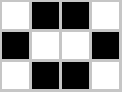
\includegraphics[height=.125\linewidth]{./images/beehive.png}
	\caption{Configuración inicial colmena.}
	\label{fig:beehive}
\end{figure} 
\begin{figure}[H]
	\centering
	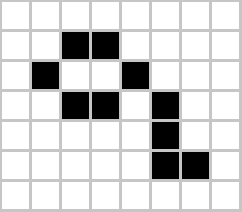
\includegraphics[height=.15\linewidth]{./images/beehive_with_tail.png}
	\caption{Configuración inicial colmena con cola.}
	\label{fig:beehive_tail}
\end{figure} 
\begin{figure}[H]
	\centering
	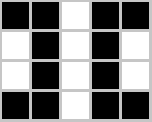
\includegraphics[height=.15\linewidth]{./images/table_on_table.png}
	\caption{Configuración inicial mesa frente a mesa.}
	\label{fig:table_on_table}
\end{figure} 

\begin{defi}
Una vida pseudo inmóvil es una vida inmóvil que puede ser particionada en vidas inmóviles independientes, es decir, la estabilidad de una de ellas no depende de la presencia de las otras. Además debe de existir al menos una célula muerta por superpoblación (más de tres vecinos vivos) que al particionar en vidas inmóviles independientes la célula continúe muerta por soledad (menos de tres vecinos vivos).
\end{defi}

Las vidas inmóviles que particionan a una vida pseudo inmóvil pueden ser a su vez vidas pseudo inmóviles \ref{fig:bisnake} o vidas inmóviles estrictas \ref{fig:biblock}. Notar que una vida inmóvil puede estar formada por varias vidas inmóviles y aún así ser una vida estrictamente inmóvil (y no pseudo inmóvil), si éstas dependen entre sí para mantener su estabilidad \ref{fig:table_on_table}.

\begin{figure}[H]
	\centering
	
\includegraphics[height=.125\linewidth]{./images/biblock.png}
	\caption{Configuración inicial bibloque.}
	\label{fig:biblock}
\end{figure} 

\begin{figure}[H]
	\centering
	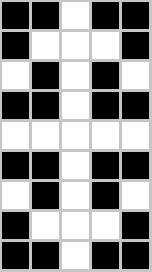
\includegraphics[height=.3\linewidth]{./images/bisnake.png}
	\caption{Configuración inicial que puede ser particionada en dos vidas pseudo inmóviles.}
	\label{fig:bisnake}
\end{figure} 


\begin{defi}
Una vida quasi inmóvil es una vida inmóvil que puede ser particionada en vidas inmóviles independientes, es decir, la estabilidad de una de ellas no depende de la presencia de las otras. Además existen células que tanto en la configuración inicial como en las vidas inmóviles independientes se mantengan muertas por soledad (menos de tres vecinos vivos). 
\end{defi}

Notar que la figura \ref{fig:biblock} no es una vida quasi inmóvil y sin embargo \ref{fig:bimoved} sí. Este tipo de vida inmóvil está habitualmente formada por dos vidas inmóviles que comparten una diagonal.

\begin{figure}[H]
	\centering
	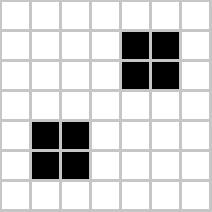
\includegraphics[height=.2\linewidth]{./images/bimoved.png}
	\caption{Configuración inicial que en el centro tiene una célula que se mantiene muerta por soledad tanto en las vidas inmóviles independientes como en el total.}
	\label{fig:bimoved}
\end{figure} 

Por último, cabría preguntarse el problema de dado un número finito de células, ¿cuántas vidas inmóviles existen? Dicho problema ha sido resuelto para vidas inmóviles estrictas y pseudo inmóviles de hasta 32 células, como se puede consultar en \cite{countStillLifes} y en \cite{countPseudoStillLifes}.

\subsection{Osciladores}

\begin{defi}
Un oscilador es una configuración inicial $z$ finita y no vacía que se repite tras la aplicación de $k$ veces de la función de transición global, esto es, fijado $n\in\mathds{N}$, se verifica que existe $k>1, \in\mathds{N}$ tal que $C^n_t(z) = C^n_{t+k}(z)$ para todo $t \leq n-k$ y diremos que $k$ es el periodo del oscilador.
\end{defi}

Notar que se exige que el periodo de oscilación sea estrictamente superior a la unidad, para evitar que la categoría de las vidas inmóviles esté contenidas dentro de la de los osciladores. 

\begin{figure}[H]
	\centering
	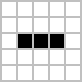
\includegraphics[height=.125\linewidth]{./images/blinker.png}
	\caption{El oscilador más pequeño de periodo dos.}
	\label{fig:blinker}
\end{figure} 

\subsection{Naves espaciales}

\begin{defi}
Una  nave espacial es una configuración inicial $z$ finita y no vacía que se repite tras la aplicación de $k$ veces de la función de transición global pero en una posición distinta, esto es, fijado $n\in\mathds{N}$, se verifica que existen $k\in\mathds{N}$ y una traslación distinta de la identidad, $\phi:\mathds{Z}^2\to\mathds{Z}^2$, tal que $C^n_t(z) = \phi(C^n_{t+k}(z))$ para todo $t \leq n-k$ y diremos que $k$ es el periodo de la nave espacial.
\end{defi}

Notar que se exige que la traslación $\phi$ sea distinta a la identidad y $k>1$, para evitar que la categoría de los osciladores esté contenida dentro de la de las naves espaciales.

Si la configuración se desplaza $x$ unidades horizontalmente e $y$ unidades verticalmente cada periodo de longitud $k$ la velocidad de desplazamiento de la nave espacial es $\max\{|x|,|y|\}c/k$ con pendiente $x/y$, siendo la velocidad máxima teórica conocida como \textit{velocidad de la luz} $c=1$, esto es, un desplazamiento por cada aplicación de la función de transición global. Según \cite{pendienteNaves} existe una nave espacial en el juego de vida de Conway para cada pendiente racional.

\begin{figure}[H]
	\centering
	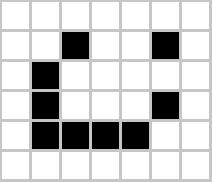
\includegraphics[height=.15\linewidth]{./images/lightweightspaceship.png}
	\caption{Nave espacial más pequeña conocida de velocidad $c/2$, su desplazamiento es paralelo a uno de los ejes de coordenadas cartesianos.}
	\label{fig:lightweightspaceship}
\end{figure} 
\begin{figure}[H]
	\centering
	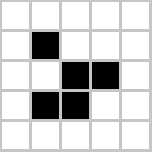
\includegraphics[height=.15\linewidth]{./images/glider.png}
	\caption{Nave espacial más pequeña conocida de velocidad $c/4$, su desplazamiento es diagonal a los ejes cartesianos de coordenadas.}
	\label{fig:glider}
\end{figure} 

\subsection{Características medidas sobre las simulaciones}

Dado el carácter aleatorio del juego de vida $\alpha$-asíncrono emplearemos los fundamentos de Monte Carlo expuestos en la sección \ref{MonteCarlo} para medir los parámetros de interés que a continuación expondremos. Dada una configuración inicial $z$ de las categorías expuestas en la sección \ref{zoo}, realizaremos múltiples simulaciones del juego de vida de Conway $\alpha$-asíncrono de duración $n=100$. Nuestras variables de interés son:

\begin{itemize}
\item Crecimiento de la población de células de la configuración inicial: dispondremos de dos herramientas para medir el número de células. Estudiaremos la evolución del número de células en cada etapa y la evolución del área rectángulo de menor tamaño que contenga a todas las células de cada etapa.
\item Tasa de cambio de la configuración inicial: emplearemos el concepto de temperatura, que es el porcentaje medio el número de células que nacen o mueren por generación.
\item Distribución de las células en cúmulos: contabilizaremos el número de cúmulos por cada generación, entendiendo por cúmulo al mayor conjunto de células cuyo vecindario no es disjunto, es decir, en un cúmulo cada célula del mismo está contenido en el vecindario de otra célula del cúmulo.
\end{itemize}

Estas variables serán medidas para distintos valores de $\alpha$ con el fin de estudiar el efecto de la aleatoriedad en las configuraciones iniciales. Notar que debido a que no se conoce a priori el número de simulaciones a partir de la cual es posible aplicar el teorema central del límite para deducir la distribución límite de la suma de variables aleatorias, el número de simulaciones que realizaremos podrá variar de una configuración inicial a otra.

% Características a medir si sobra tiempo: simulaciones utilizando cadenas de markov y métodos de monte carlo


\end{document}